\chapter{Méthodes expérimentales}

\section{pix2pix avec PASCAL}

Nous avons implémenté le modèle pix2pix sur un sous ensemble de données d'image prévenant de la dataset Pascal, cet ensemble contient 2913 paires d'images (image d'origine et segmenté) sur 20 classes différentes :
\begin{itemize}
	\item Personne : personne 
	\item Animal : oiseau, chat, vache, chien, cheval, mouton
	\item Véhicule : avion, bicyclette, bateau, bus, voiture, moto, train
	\item Intérieur : bouteille, chaise, table à manger, plante en pot, canapé, télévision/moniteur
\end{itemize}

Comme la plupart des utilisateurs de pix2pix sont basées sur des jeux de données à une classe, tels que le visage, la façade…etc. Nous menons des expériences sur le jeu de données qui a une scène plus complexe, qui souvent contient plus d'une classe dans une image, par exemple :


\begin{figure}[H] 
	\centering 
	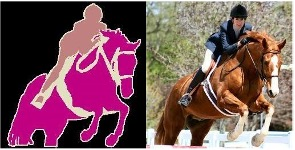
\includegraphics[width=0.7\textwidth]{./resources/img/im_pascal.jpg} %插入图片,[]中设置图片大小,{}中是图片文件名
	\caption{Image segmenté et image d'origine contenant une personne et un cheval} %最终文档中希望显示的图片标题
	\label{Fig4_1} %用于文内引用的标签
\end{figure}


\newpage
 Nous avons effectué notre expérience sur le pix2pix en trois parties :
 
 \begin{enumerate}[label=(\alph*)]
 	\item Sur les voitures
 	
 	Tout d'abord, nous avons mené notre expérience sur le sous-ensemble de données qui contient principalement que des voitures. Après 200 époques d'apprentissage avec une taille de lot de 1, le modèle est capable de générer le profil général d'une voiture, et il est capable de remarquer la position des pneus et des fenêtres. De plus, comme la plupart des voitures dans l'ensemble du jeu de données sont noirs et rouge, et pix2pix est un GAN basé sur la théorie statique. Les voitures générées sont principalement en noir avec un mélange de rouge. (Exemple en annexe).
 	
 	
 	\item Sur toute les images avec leurs arrière-plans
 	
 	Deuxièmement nous avons nous avons mené l'expérience avec toute des images, et la plupart de ces images présente des scènes complexes avec plusieurs classe en même temps. Après 400 époques d'apprentissage avec une taille de lot de 1, Malgré que la classe personne est la plus redondante dans nos images, il est difficile de générer une personne réelle à partir de l'image d'entrée. Et pour certaines classes simples comme les avions, vélos, bus et les bateaux qui apparaissent souvent dans des scènes monotones (ciel, routes, mer…etc.), le modèle est capable de générer un objet très similaires à un objet réel. (Exemple en annexe).
 	
 	\item Sur toute les images sans leurs arrière-plans
 	
 	
 	Enfin, nous avons expérimenté sur l'ensemble des images en augmentant le nombre des images par la duplication (miroir et rotation) et en enlevant l'arrière-plan afin de savoir si l'arrière-plan influence. L'une des raisons est que les scènes ou les personnes apparaissent sont très variées et après 300 époques d'entrainement avec une taille de lot de 1, nous avons générer des images (Exemple en annexe). Et nous avons observé qu'il n'y a pas de d'amélioration par rapport à l'étape avec les images contenants l'arrière-plan.
 	
 \end{enumerate}

À la fin de ces expériences nous avons dessiné les graphes de loss afin d'observer le comportement de la loss du générateur et notamment la loss du discriminateur. Nous notons que le D{\_}real avec la ligne verte signifie la loss du discriminateur pour les images réelles, le D{\_}fake signifie la loss du discriminateur pour les images fausses g.n.r.es enfin nous avons G{\_}GAN qui signifie la loss du générateur pour les images fausses. Nous notons aussi que la stabilité de notre modèle est liée à la stabilité des loss de D{\_}real, D{\_}fake et G{\_}GAN.

\begin{figure}[H] 
	\centering 
	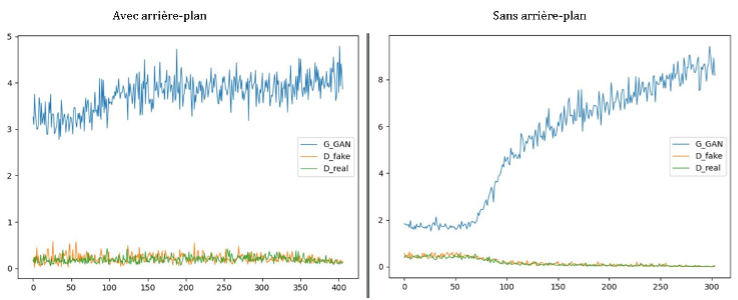
\includegraphics[width=1.0\textwidth]{./resources/img/im_pascal_loss.png} %插入图片,[]中设置图片大小,{}中是图片文件名
	\caption{Graphe de loss de pix2pix avec les images contenant un arrière-plan et non.} %最终文档中希望显示的图片标题
	\label{Fig4_2} %用于文内引用的标签
\end{figure}

Nous remarquant que notre modèle avec des images contenant un arrière-plan est stable car G{\_}GAN, D{\_}fake et D{\_}real sont stable. Et pour le modèle avec les images sans arrière-plan, il est stable jusqu'à l'époque 75, puis devient instable car la loss de G{\_}GAN augment énormément.
Nous avons aussi appliqué le modèle avec l'arrière-plan sur des images qui ne contiennent pas d'arrière-plan afin le modèle permet de générer un arrière-plan presque parfait pour certaines classes par exemple pour les avions il génère le ciel, pour les animaux il génère la verdure (Exemple en annexe).
